%!TEX root = jsba_main.tex
% Results

\section{Results}
\label{sec:res}

This Section reports and presents the findings of the query execution time measurements. Appendix~\ref{app:queries} lists all queries that were executed
for each implementation without flexible answering and Appendix~\ref{app:flexqueries} lists the queries that were executed flexibly with the previously
described query generalization (cf. Section~\ref{sec:meth_fqa_qgen}). For both developed approaches (cf. Section~\ref{sec:impl_alter}), different horizontal
fragmentations based on the underlying clustering were also investigated. The different fragmentations are caused by restricting the size of the term set 
(cf. Appendix~\ref{app:terms}) to only the first 10 or 30 terms or all 100 terms. Furthermore, the size of the database was scaled for each implementation with
a scaling factor (SF) of 1 up to 10000 that is multiplied with the default number of \verb!INFO! tuples (50) and the default number of \verb!ILL! tuples (100),
i.e. on average each patient has two diseases.
The following bar charts display the average query execution time of 10 executions of a query in milliseconds on the y-axis in dependence on the different 
scaling factors shown on the x-axis. In the legend, the different implementations are listed whereas
"Materialized" and "Partitions" refer to the first (cf. Section~\ref{sec:impl_alter_mater}) and second (cf. Section~\ref{sec:impl_alter_partnum}) approach,
respectively, and the attached numbers indicate the size of the underlying term set (10, 30 or 100) and "Reference" refers to the reference implementation 
(cf. Section~\ref{sec:impl_refimpl}).

Figure~\ref{fig:query1} shows the average execution time of $Q_1$. As this query is selecting the average age of all persons in the database, 
there can not be performed any intelligent execution based on the similarity metric together with the clustering of the data. Only for the last two scaling
factors, there is a noticeable increase in the execution time because the amount of data to be scanned also increased. The outlier (Partitions100, SF=10000)
might be caused by an accidentally imbalanced or adverse distribution of the data across the partitions in contrast to the other implementations.
\begin{figure}[h]
    \centering
    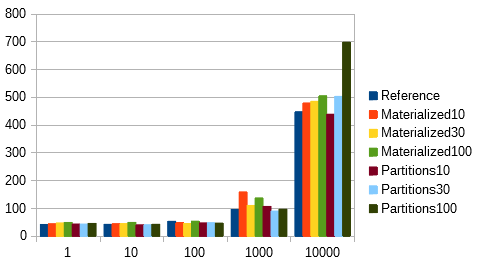
\includegraphics[scale=0.8]{charts/Query1.png}
    \caption{Average query execution time in milliseconds of $Q_1$ (Appendix~\ref{app:queries})}
    \label{fig:query1}
\end{figure}

For the second query, $Q_2$, the reference implementation's average query execution time took with increasing relation sizes always longer than any
implementation of the developed approaches (cf. Figure~\ref{fig:query2}). Even for the smaller scaling factors except for the SF of 1, the execution time was
slightly longer and for the highest scaling factor the execution time of almost five seconds was approximately 50 times as long as the other execution times.
This is because the reference implementation is unlike the developed approaches not capable of answering queries similarity-based as it lacks the
clustering-based fragmentation for the relaxation attribute. The developed approaches, on the contrary, are able to perform similarity-based query answering 
(cf. Section~\ref{sec:meth_sbqa}) for this query as it contains a selection condition on the relaxation attribute. Thus after identification of the relevant
fragment and query rewriting, the query execution is optimized.

\begin{figure}[h]
    \centering
    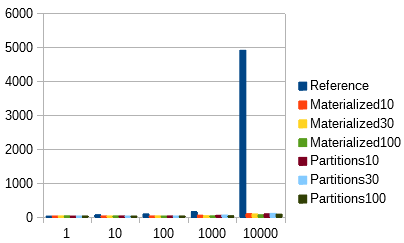
\includegraphics[scale=0.9]{charts/Query2.png}
    \caption{Average query execution time of $Q_2$ (Appendix~\ref{app:queries})}
    \label{fig:query2}
\end{figure}

To demonstrate the small differences in the query execution time for the other approaches, the next chart (Figure~\ref{fig:query2withoutref}) plots the same
execution times without the measurements of the reference implementation that are beyond the scope. Two interesting things illustrated in this chart are that,
firstly, both approaches approximately coincide with the execution times and, secondly, both approaches have their fastest execution times (SF=1000 and
SF=10000) for the whole term set compared to the other term set sizes. This is due to the fact that if there are less terms underlying the clustering, then 
more patients will have a tuple in the \verb!ILL! relation with the disease term \verb!'Liver Failure'! as the data is generated completely randomly and
diseases are picked randomly from the chosen term set. This results in more tuples matching the selection condition and also more tuples that have to be joined,
whereas the join is still pretty fast due to collocation, but a presumably bigger result set has to be transferred back to the client.

\begin{figure}[h]
    \centering
    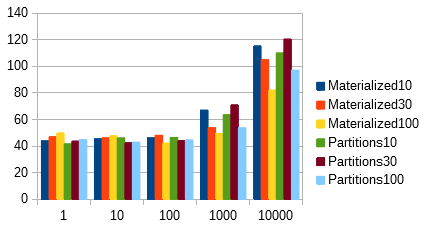
\includegraphics[scale=0.9]{charts/Query2WithoutReference.png}
    \caption{Average query execution time of $Q_2$ (Appendix~\ref{app:queries}) without reference implementation}
    \label{fig:query2withoutref}
\end{figure}


The situation for query 3 from Appendix~\ref{app:queries} is almost the same as for query 2 because as depicted in Figure~\ref{fig:query3} the average execution
time of the query was multiple times higher for the reference implementation, too. Here, the measurement was even approximately 600 times higher for the biggest
database size (SF=10000). In comparison to the previous query, this behaviour can be explained by the fact that the relation \verb!ILL! is joined with itself in
the query's \verb!FROM! clause instead of only once with the \verb!INFO! relation. In case of the distributed data, this query answer calculation is 
computationally expensive. One possible execution for the DDBS is to separately collect all tuples from the \verb!ILL! relation that either satisfy the first 
selection condition (\verb!i1.disease = 'Liver Failure'!) or the second one (\verb!i1.disease = 'Hemoptysis'!) on one server in two sets that are joined after 
the collection via the shared attribute (\verb!i1.id = i2.id!). This join is not explicitly formulated in the query but it can be concluded implicitly from the 
transitivity of the "\verb!=!-chain" in the \verb!WHERE! clause. In the last step, the joined tuples have to be joined again with the \verb!INFO! relation that 
is distributed and requires for transferring tuples between the servers. A more efficient execution is achieved by pushing down the join with the \verb!INFO!
tuples as the collocation allows for a local join and avoids costly data transfer.
\begin{figure}[h]
    \centering
    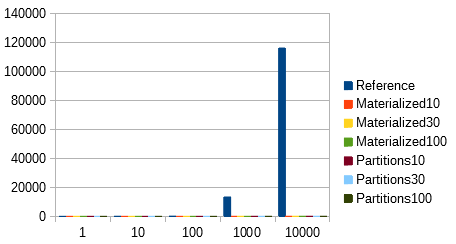
\includegraphics[scale=0.9]{charts/Query3.png}
    \caption{Average query execution time of $Q_3$ (Appendix~\ref{app:queries})}
    \label{fig:query3}
\end{figure}


Figure~\ref{fig:query3withoutref} depicts the same time measurements as before without the execution times of the reference implementation which are again beyond
the scope. Here, one can see that the average execution time of $Q_3$ has an equal length for the three smallest scaling factors and only increases for the
biggest two factors. The main reason for this behaviour is first of all the increased amount of data. But as the comparison to Figure~\ref{fig:query2withoutref}
reveals, the query execution of $Q_3$ takes around 100ms longer (SF=10000) than the execution of $Q_2$. This is due to the fact that the similarity-based query
answering technique (cf. Section~\ref{sec:meth_sbqa}) identifies two fragments, one corresponding to the cluster where the disease term "Liver Failure" belongs
to and one corresponding to the cluster where the disease term "Hemoptysis" belongs to, where, in contrast to this, for answering $Q_2$ the former suffices. 
Furthermore, the tuples of those two fragments need to be joined in order to provide the correct result set which can be performed locally in the optimal case,
i.e. when both fragments are hosted by the same server, but involves data transfer between the two servers if the fragments do not reside at the same server.
Due to this reasons, the execution of $Q_3$ is slightly slower than $Q_2$ but still the developed approaches outperform the reference implementation.
\begin{figure}[h]
    \centering
    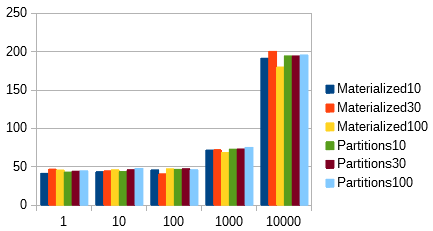
\includegraphics[scale=0.9]{charts/Query3WithoutReference.png}
    \caption{Average query execution time of $Q_3$ (Appendix~\ref{app:queries}) without reference implementation}
    \label{fig:query3withoutref}
\end{figure}


The average execution times for $Q_4$ (Figure~\ref{fig:query4}) and $Q_5$ (Figure~\ref{fig:query5}) show again only few differences between all 
implementations for the smaller database sizes. But as the size is increased by a factor of 10000, both queries are executed approximately 5 to 7 times as long 
in the materialized fragment approach than compared to the reference implementation whereas the other approach is only slightly slower (up to twice as long).
Because of the requirement to rewrite the queries in the materialized fragment approach according to the localization program of the underlying fragmentation,
the average execution time takes significantly longer in this approach as the rewritten query comprises one subquery per fragment that are all connected in a 
big SQL \verb!UNION!, e.g. for $n$ fragments the rewritten query $Q_{rewritten}$ is
\begin{verbatim}
    (SELECT ... FROM ILL_0 i, INFO_0 p WHERE ...)
    UNION
    (SELECT ... FROM ILL_1 i, INFO_1 p WHERE ...)
    UNION
    ...
    UNION
    (SELECT ... FROM ILL_n i, INFO_n p WHERE ...)
\end{verbatim}
(cf. Example~\ref{sec:theo_dqp_exmp2}). The stair-like appearance of the three corresponding bars (orange, yellow, green) mirror the total number of clusters 
and fragments of the relations from the underlying clustering-based fragmentation This complex and long query can not be executed as fast as the non-rewritten
queries. A reason why the query execution in the partition number approach is a little bit slower than the reference implementation could be a disadvantageous
distribution of data to the different fragments leading to a non-optimal performance when executing the query. Additionally, the by \citetalias{Ignite} provided
automatic partitioning and distribution of the data can be handled in a more balanced way as the DDBS strives to equalize the load on all participating nodes
yielding a more balanced data distribution that might be more advantageous for execution of the queries in comparison to the clustering-influenced distribution
of the developed approaches.
\begin{figure}[h]
    \centering
    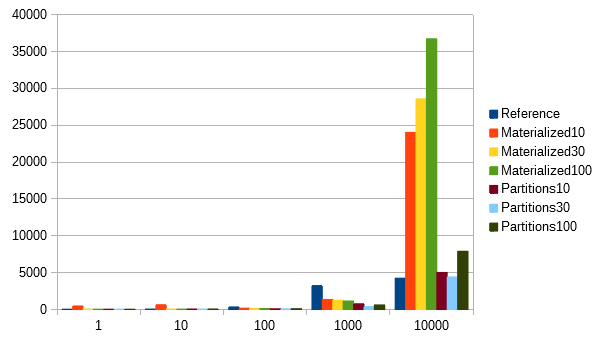
\includegraphics[scale=0.8]{charts/Query4.png}
    \caption{Average query execution time of $Q_4$ (Appendix~\ref{app:queries})}
    \label{fig:query4}
\end{figure}

\begin{figure}[h]
    \centering
    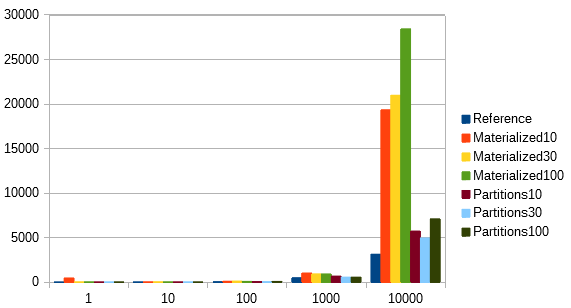
\includegraphics[scale=0.8]{charts/Query5.png}
    \caption{Average query execution time of $Q_5$ (Appendix~\ref{app:queries})}
    \label{fig:query5}
\end{figure}



The time measurements for the execution of $Q_6$ are illustrated in Figure~\ref{fig:query6}. The execution of this query was only investigated for the scaling 
factors 1, 10 and 100 as for the bigger factors the query execution time exceeded the timeout threshold of 10 minutes. The interesting points here are firstly
coincidence of the measurements for the reference implementation with the measurements of the partition number approach and secondly the stair-like shape of
the bars that belong to execution times of the materialized fragment approach as already seen before for $Q_4$ and $Q_5$. The higher execution times for the
materialized fragment approach are caused by the complexity of the rewritten query that looks very similar to the previously sketched $Q_{rewritten}$ but as the
initial query contains a join of the relation \verb!ILL! with itself the corresponding localization program has to consider all pairs of two materialized
\verb!ILL! fragments, i.e. for each materialized fragment table there is a subquery that has the same structure as $Q_{rewritten}$ with an additional join of
that certain fragment table and all the subqueries, which are unions of subqueries themselves, are aggregated by \verb!UNION!s to one final query. The impact of
this nesting of subqueries connected by unions on the query execution performance increases exponentially with the number of joined relations.

\begin{figure}[h]
    \centering
    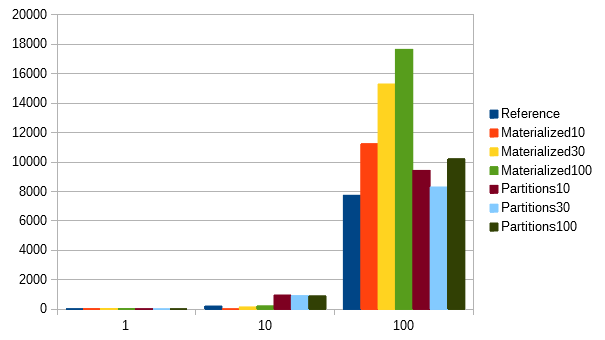
\includegraphics[scale=0.8]{charts/Query6.png}
    \caption{Average query execution time of $Q_6$ (Appendix~\ref{app:queries})}
    \label{fig:query6}
\end{figure}


\todo[inline]{FAQ}